\documentclass[border=3pt]{standalone}
\usepackage{amsmath,amssymb}
\usepackage{tikz}
\usetikzlibrary{arrows.meta,positioning,calc,backgrounds,fit}
\begin{document}
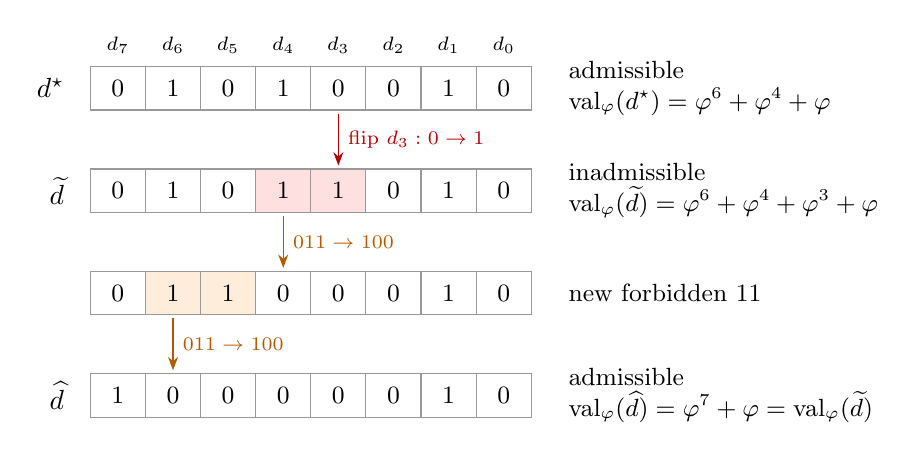
\begin{tikzpicture}[x=0.7cm,y=1cm,>=Stealth,
  cell/.style={draw=black!40,minimum width=0.7cm,
    minimum height=0.55cm,inner sep=0pt,font=\small},
  info/.style={anchor=west,align=left,font=\small}]
\foreach \p in {0,...,7}{
  \node[font=\scriptsize] at (\p,0.55) {\(d_{\the\numexpr7-\p\relax}\)};
}
\foreach \row/\digits in {
  0/{0,1,0,1,0,0,1,0},
  1/{0,1,0,1,1,0,1,0},
  2/{0,1,1,0,0,0,1,0},
  3/{1,0,0,0,0,0,1,0}}{
  \foreach \d [count=\p from 0] in \digits{
    \node[cell,fill=white] at (\p,-1.3*\row) {\d};
  }
}
\foreach \p in {3,4}{
  \node[cell,fill=red!12] at (\p,-1.3) {1};
}
\foreach \p in {1,2}{
  \node[cell,fill=orange!14] at (\p,-2.6) {1};
}
\node[anchor=east] at (-0.8,0) {\(d^\star\)};
\node[anchor=east] at (-0.8,-1.3) {\(\widetilde d\)};
\node[anchor=east] at (-0.8,-3.9) {\(\widehat d\)};
\node[info] at (8,0)
  {admissible\\\(\operatorname{val}_\varphi(d^\star)=
    \varphi^6+\varphi^4+\varphi\)};
\node[info] at (8,-1.3)
  {inadmissible\\\(\operatorname{val}_\varphi(\widetilde d)=
    \varphi^6+\varphi^4+\varphi^3+\varphi\)};
\node[info] at (8,-2.6) {new forbidden \(11\)};
\node[info] at (8,-3.9)
  {admissible\\\(\operatorname{val}_\varphi(\widehat d)=
    \varphi^7+\varphi=\operatorname{val}_\varphi(\widetilde d)\)};
\draw[->,red!70!black] (4,-0.32)--(4,-0.98)
  node[midway,right,font=\scriptsize] {flip \(d_3:0\to1\)};
\draw[->,orange!70!black] (3,-1.62)--(3,-2.28)
  node[midway,right,font=\scriptsize] {\(011\to100\)};
\draw[->,orange!70!black] (1,-2.92)--(1,-3.58)
  node[midway,right,font=\scriptsize] {\(011\to100\)};
\end{tikzpicture}
\end{document}
